\chapter{Fundamentação Teórica} \label{cap:cap2}

Este Capítulo relaciona os conceitos e as tecnologias envolvidas no desenvolvimento do ambiente de treinamento proposto. 

\section{Anestesias Regionais}

Anestesias são atualmente usadas em diversos procedimentos cirúrgicos na medicina tradicional com o intuito de bloquear temporariamente a capacidade do cérebro de reconhecer um estímulo doloroso. Esta prática visa permitir a execução de procedimentos invasivos por parte do médico enquanto mantém o conforto e a tranquilidade do paciente. A anestesia regional é um procedimento usado em cirurgias onde o paciente pode permanecer acordado. Este tipo de anestesia bloqueia a dor em apenas uma determinada região do corpo, como um braço, uma perna ou toda região inferior do corpo, abaixo do abdômen \cite{Pinheiro2018}.

Os dois tipos de anestesias regionais mais usados são: anestesia raquidiana (ou raquianestesia, raqui), e anestesia peridural ou epidural. Estes dois tipos de anestesias também são conhecidas como anestesias de neuroeixo ou ainda bloqueio de neuroeixo \cite{Pinheiro2018}. Ambas podem ser aplicadas com pacientes sentados e inclinados para frente ou deitados de lado \cite{Anesclin2019}. 

\begin{figure}[ht!]
    \centering
    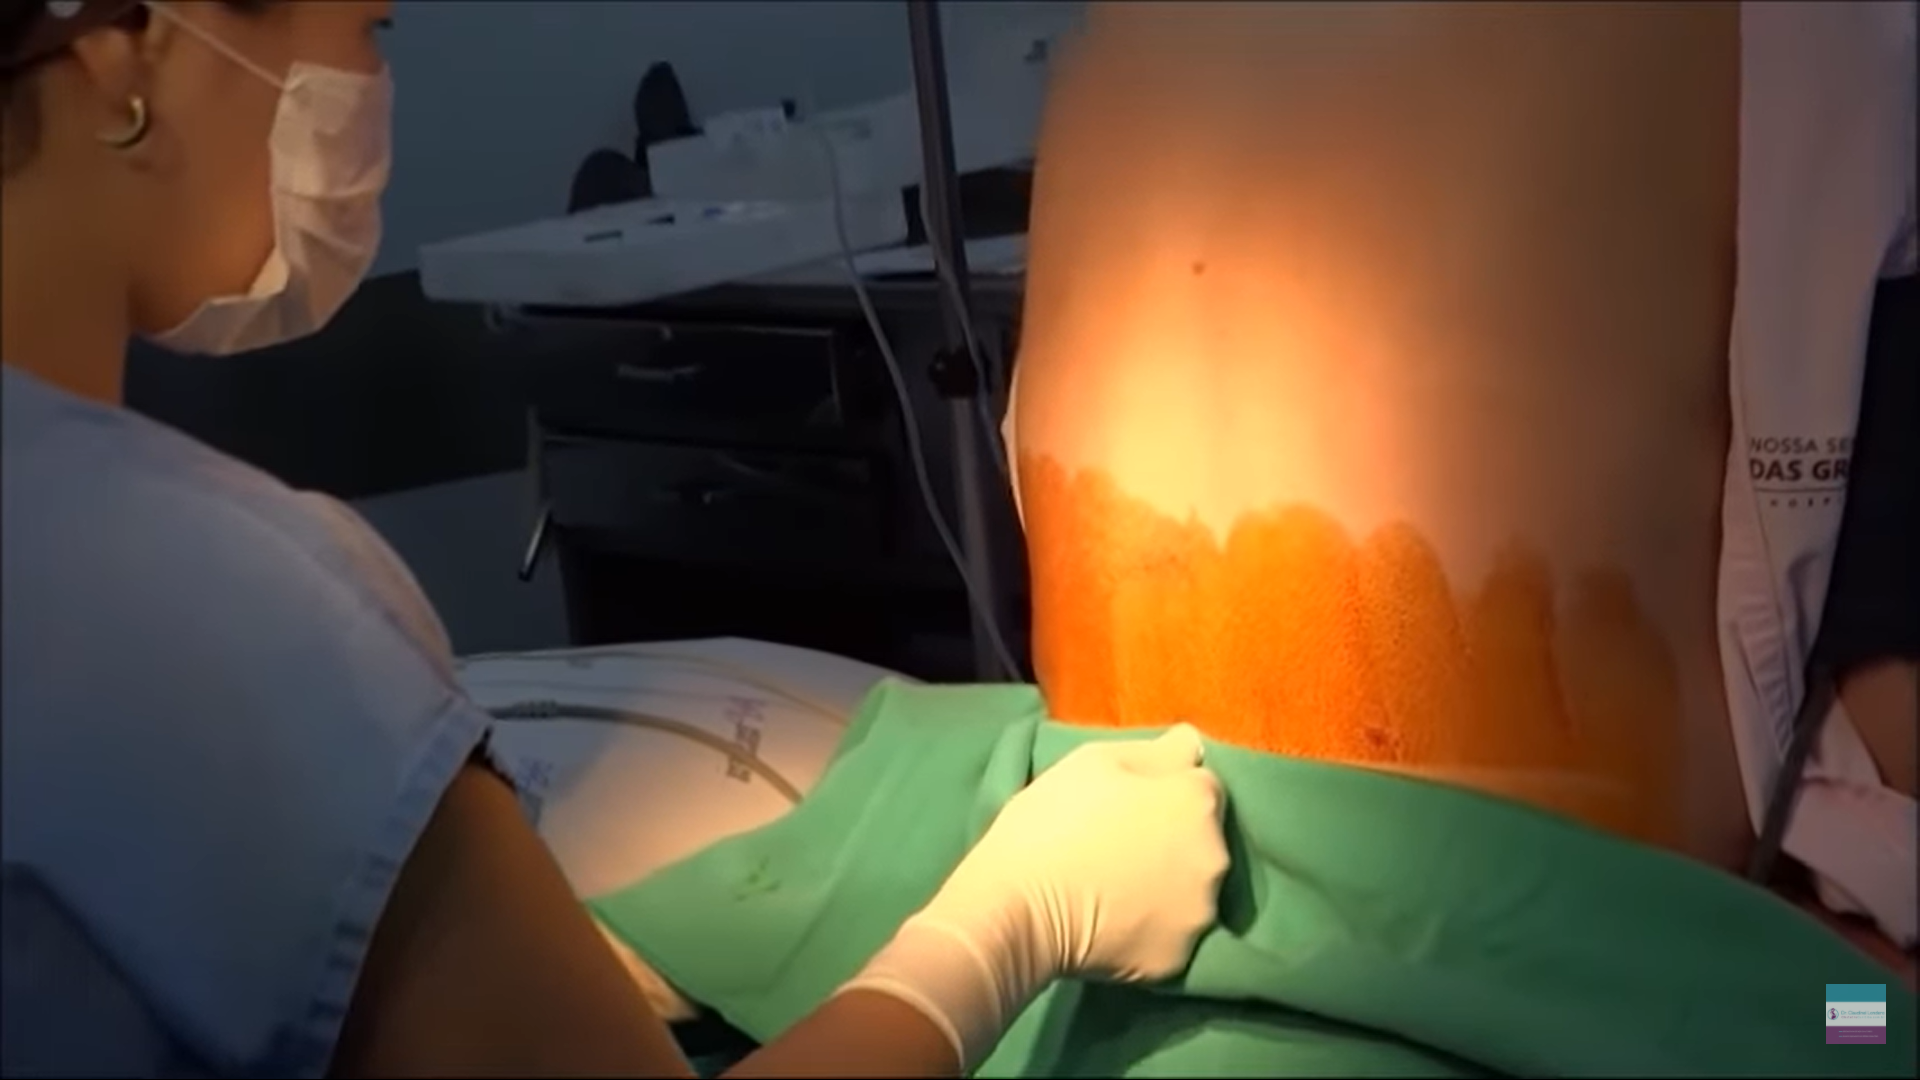
\includegraphics[width=0.6\linewidth]{capitulos/figuras/0.marcacaoPonto.png}
    \caption{Palpação para determinação do ponto de inserção da agulha \cite{Londero2018}.}
    \label{fig:marcacaoPonto}
\end{figure}

\begin{figure}[ht!]
    \centering
    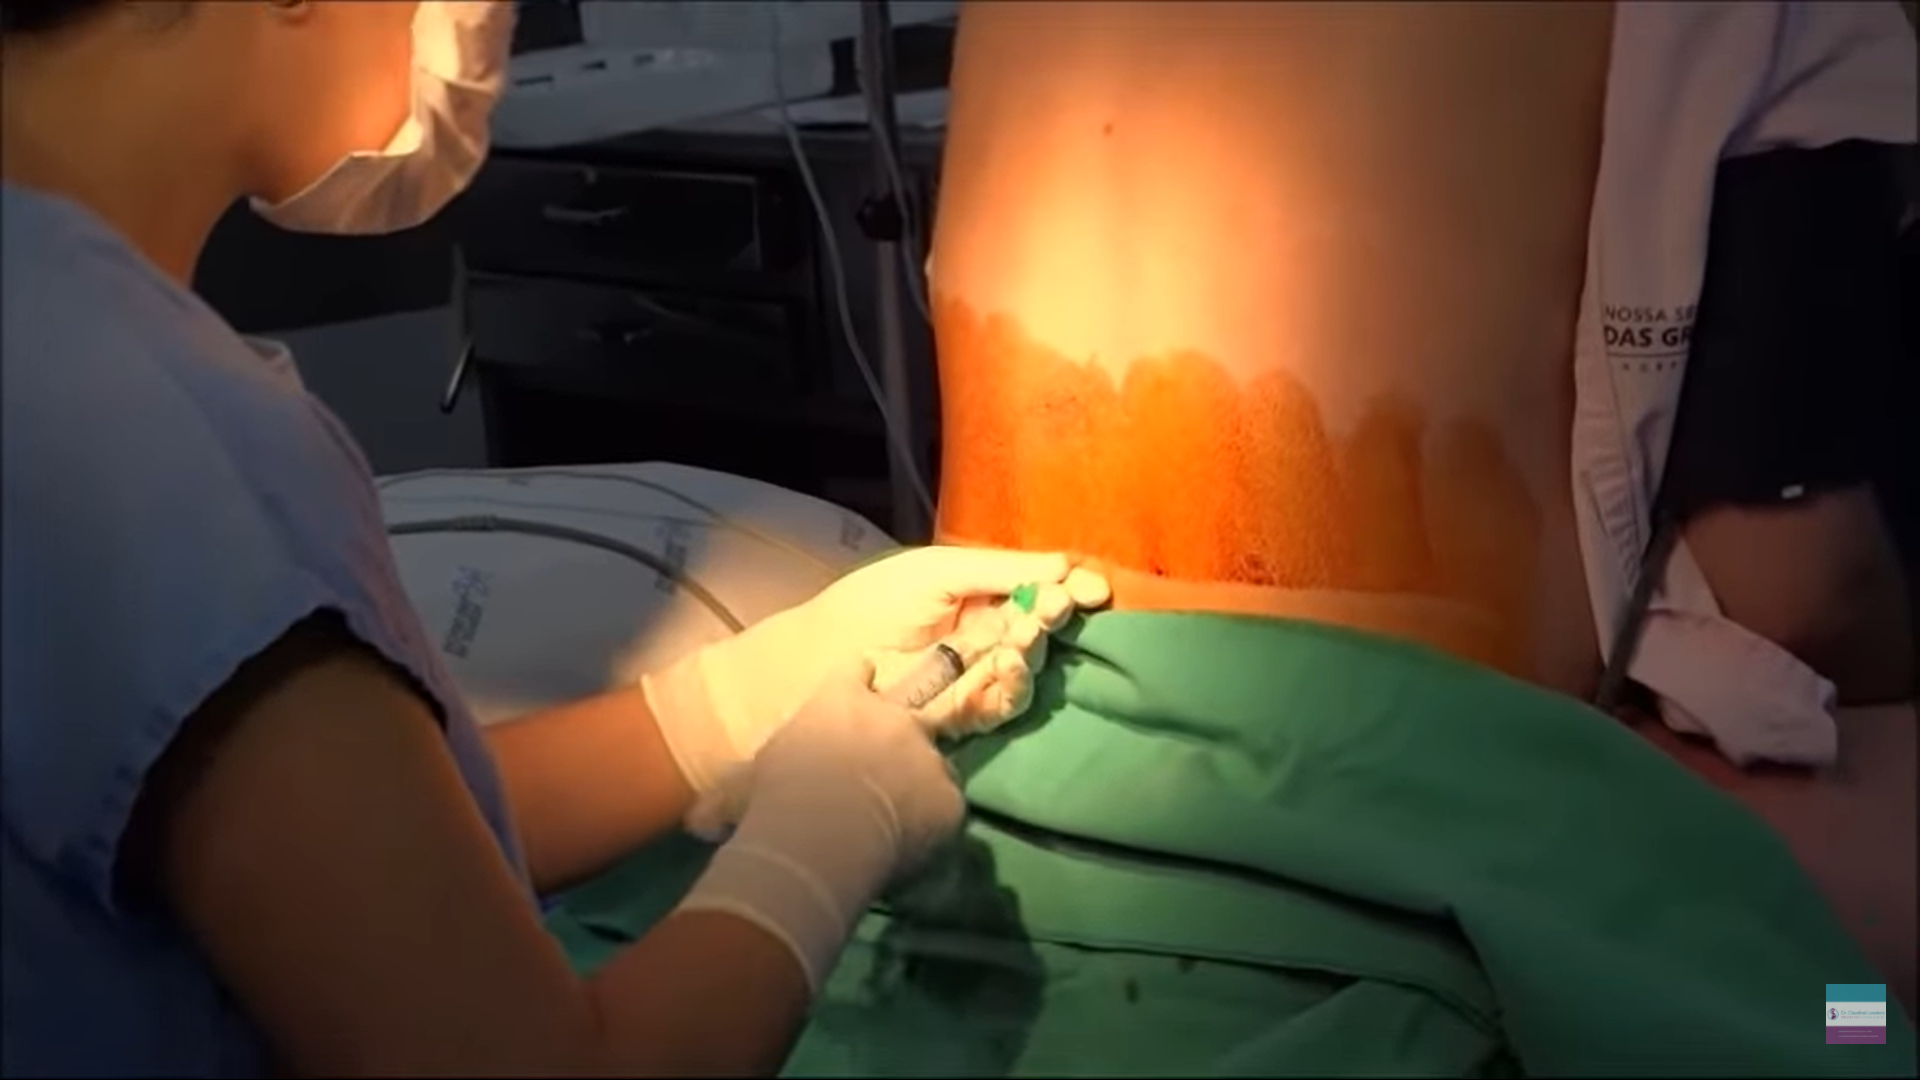
\includegraphics[width=0.6\linewidth]{capitulos/figuras/1.AnestesiaLocal.png}
    \caption{Aplicação da anestesia local \cite{Londero2018}.}
    \label{fig:anestesiaLocal}
\end{figure}

\begin{figure}[ht!]
    \centering
    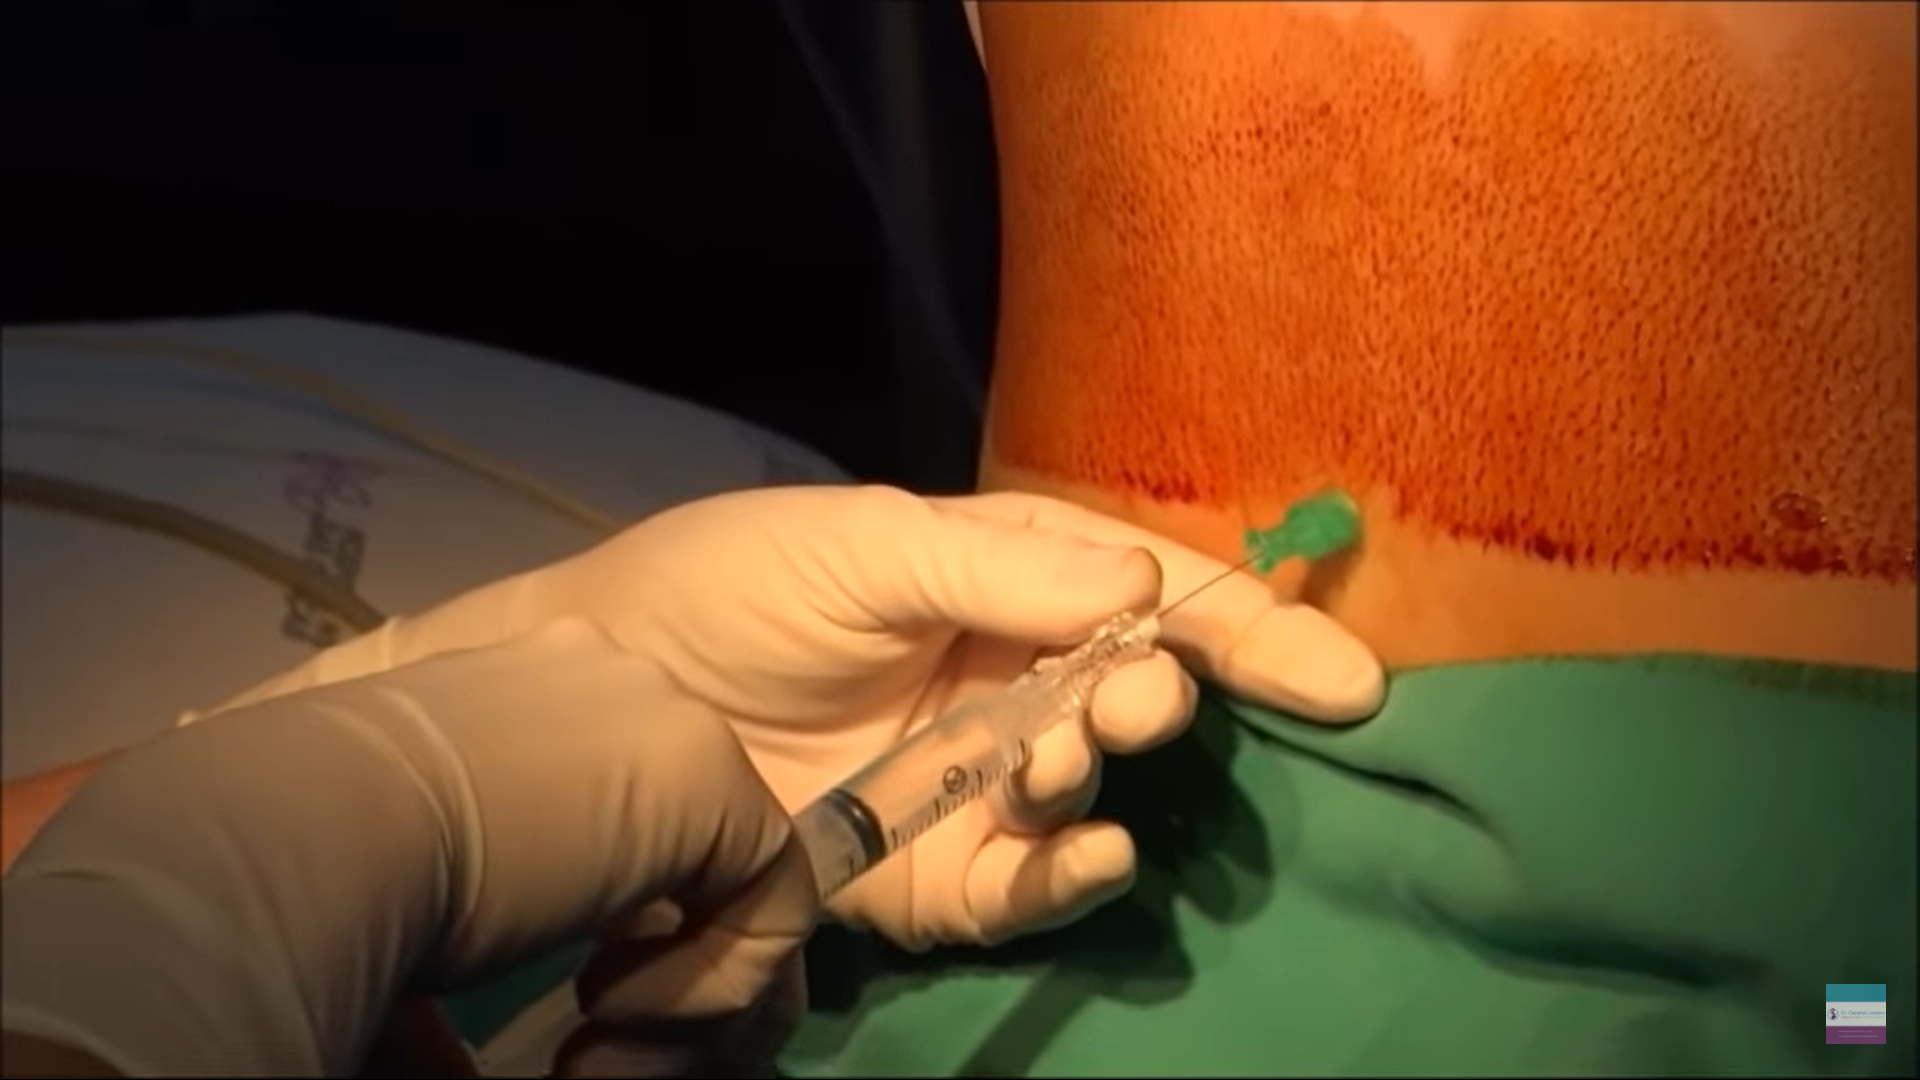
\includegraphics[width=0.6\linewidth]{capitulos/figuras/4.InjecaoAnestesico.png}
    \caption{Injeção do liquido anestésico no espaço subaracnóideo  \cite{Londero2018}.}
    \label{fig:injecaoAnestesico}
\end{figure}

Após a finalização dos procedimentos de preparação é escolhida a área onde será feita a punção através do toque da mão do médico (exemplo retirado de video na Figura~\ref{fig:marcacaoPonto}) na crista ilíaca do paciente \cite{Helayel2010,Isaacs2015}. Uma vez escolhido este ponto é feita a injeção de anestésico local (Figura~\ref{fig:anestesiaLocal}) para reduzir o desconforto na área próxima à punção \cite{Sedicias2018} Após a anestesia local é feita a inserção da agulha de punção tanto no caso da peridural como na raqui.

Existem duas principais abordagens de inserção da agulha para efetuação das anestesias regionais. Estão são denominadas mediana (do inglês \textit{midline}) e paramediana (do inglês \textit{paramedian}). A abordagem mediana é utilizada com mais frequência (96\%) \cite{Wantman2006}. Um dos motivos para o maior uso da abordagem mediana é a ausência de vasos sanguíneos no caminho da agulha nesta abordagem \cite{Bapat2015}. A abordagem paramediana é mais recomendada para pacientes idosos \cite{Ahsan-ul-Haq2005} por motivos de modificação degenerativa da coluna vertebral \cite{Boon2003} e calcificação dos ligamentos interespinhoso e supraespinhoso \cite{Wantman2006}. A abordagem paramediana também pode ser mais viável que a mediana em pacientes obesos pela dificuldade na identificação da crista ilíaca nestes pacientes. Isto por que a camada de gordura faz com que a linha média seja mais difícil de localizar através do toque do médico \cite{N.2013}. Na abordagem mediana a agulha é inserida na linha média da coluna vertebral. Na paramediana existe certa angulação entre a linha da coluna e a inserção da agulha. As duas abordagens podem ser observadas no corte transversal da coluna na Figura~\ref{fig:abordagensInsercaoAgulha}. 

\begin{figure}[ht!]
    \centering
    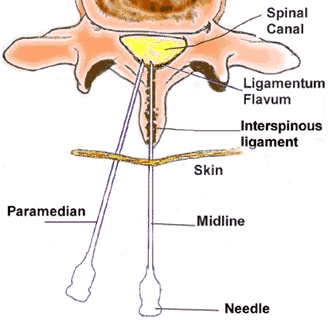
\includegraphics[width=0.6\linewidth]{capitulos/figuras/paramedian-midline-MedBroadcast-Tiff.png}
    \caption{Ilustração da abordagem mediana e paramediana para inserção de agulha \cite{MedBroadcast2018}.}
    \label{fig:abordagensInsercaoAgulha}
\end{figure}

\subsection{Anestesia Raquidiana}

Neste tipo de anestesia, uma agulha de pequeno calibre é inserida nas costas do paciente até atingir o espaço subaracnóideo (localizado após a dura-máter), dentro da coluna espinhal. Em seguida, um anestésico é injetado dentro do líquido cérebro espinhal (\textit{líquor}), produzindo dormência temporária e relaxamento muscular (Figura~\ref{fig:injecaoAnestesico}). Anestesias raquidianas são aplicadas de forma mais frequente em espaços intervertebrais abaixo da segunda vértebra lombar (L2), normalmente entre a L3 e L4 \cite{Wikipedia2019, Londero2018}. A Figura~\ref{fig:camadasPuncaoLombar} ilustra em um corte sagital da coluna as diferentes camadas que são cruzadas por uma agulha durante o procedimento de punção lombar até chegar ao espaço subaracnóideo. Considerando as duas abordagens de inserção da agulha (mediana e paramediana) as camadas onde a agulha pode passar desde a pele até o espaço subaracnóideo são: gordura subcutânea, músculo, ligamento supraespinhoso, ligamento interespinhoso, ligamento amarelo (\textit{flavum}), espaço epidural e dura-máter. O processo espinhoso que também aparece entre a pele e o espaço subaracnóideo na Figura~\ref{fig:camadasPuncaoLombar} não foi listado, pois, por ser uma camada de osso, ela não é perfurada pela agulha e sim uma camada intransponível em relação ao processo de punção.

\begin{figure}[ht!]
    \centering
    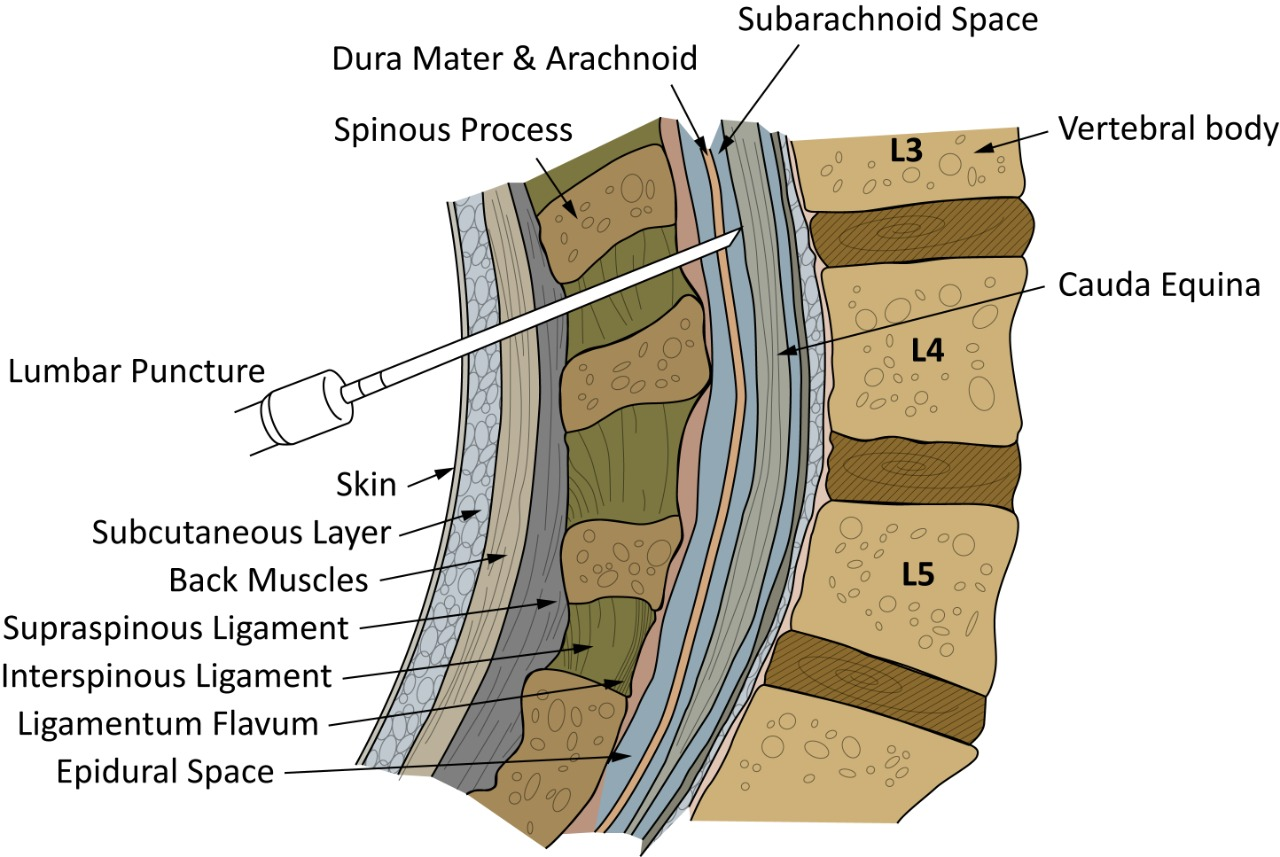
\includegraphics[width=0.6\linewidth]{capitulos/figuras/lumbar.puncture.tisssues.jpeg}
    \caption{Camadas cruzadas pela agulha numa punção lombar.}
    \label{fig:camadasPuncaoLombar}
\end{figure}

A ação do anestésico dentro da coluna espinhal é a de bloquear os nervos que passam pela coluna lombar, fazendo com que os estímulos dolorosos vindos de membros inferiores e do abdômen não cheguem ao cérebro. A raquianestesia é muito usada para procedimentos ortopédicos de membros inferiores assim como na região abdominal e cirurgias obstétricas de parto normal e cesarianas \cite{Pinheiro2018}.

A grande vantagem da anestesia raquidiana em relação a peridural é que nesta é necessário o uso de uma pequena quantidade de anestésico local. Esta característica reduz consideravelmente o risco de intoxicação por meio do elemento anestésico. Por outro lado a maior desvantagem no uso deste tipo de anestesia está na dor de cabeça que os pacientes sentem após a perfuração da dura-máter. Este sintoma é causado pela lesão na dura-máter que pode permanecer aberta por alguns dias após o procedimento, provocando perda do \textit{líquor} do espaço subaracnóideo. Com o uso de agulhas de menor diâmetro a incidência desta dor de cabeça foi consideravelmente reduzida \cite{INFOESCOLA2018}. 

\section{Realidade Virtual}

A \acrlong{RV} está presente quando se usa a tecnologia para criar a ilusão de que se está em um ambiente que não está lá ou não existe. Ela é uma aproximação da realidade experimentada por nós através dos nossos sentidos e sistemas de percepção. A nossa percepção da realidade vem através dos nossos sentidos. Portanto, uma vez apresentando aos sentidos às informações esperadas, sendo estas reais ou não, a nossa percepção da realidade irá se guiar por estes estímulos. Os sentidos mais comuns são visão, olfato, paladar, audição e tato. Porém também possuímos outros sentidos que afetam as nossas percepções do mundo, como por exemplo: o senso de equilíbrio, o sentimento de forças, pesos e deslocamentos sentidos por nossos membros \cite{VRS2018}.

Atualmente, a chamada \acrfull{RV} utiliza um computador para criar um ambiente virtual tridimensional. A intenção é a de simular uma realidade apresentando os elementos desejáveis para os sentidos do usuário, visando cumprir um objetivo através da interação de um ou mais usuários com este ambiente. Estes usuários se tornam parte deste ambiente virtual, total ou parcialmente, podendo manipular objetos ou executar um conjunto de ações \cite{VRS2018}.

A \acrshort{RV} possui uma série de usos sociais como, por exemplo, o tratamento de fobias. Há trabalhos para aracnofobia \cite{Carlin1997}, para aicmofobia ou medo de agulhas \cite{Galoustian2018}, para aerofobia ou medo de voar \cite{Rothbaum2006}, para acrofobia ou medo de altura \cite{Edwards2018} ou de forma mais geral para o medo e a ansiedade \cite{Goldman2017}. A Figura~\ref{fig:medoAltura} ilustra a aplicação para tratamento da acrofobia. Em primeiro plano a usuária com os óculos de realidade virtual e no segundo plano o ambiente virtual simulando ambientes de escadas e plataformas com fundo transparente.

\begin{figure}[ht!]
    \centering
    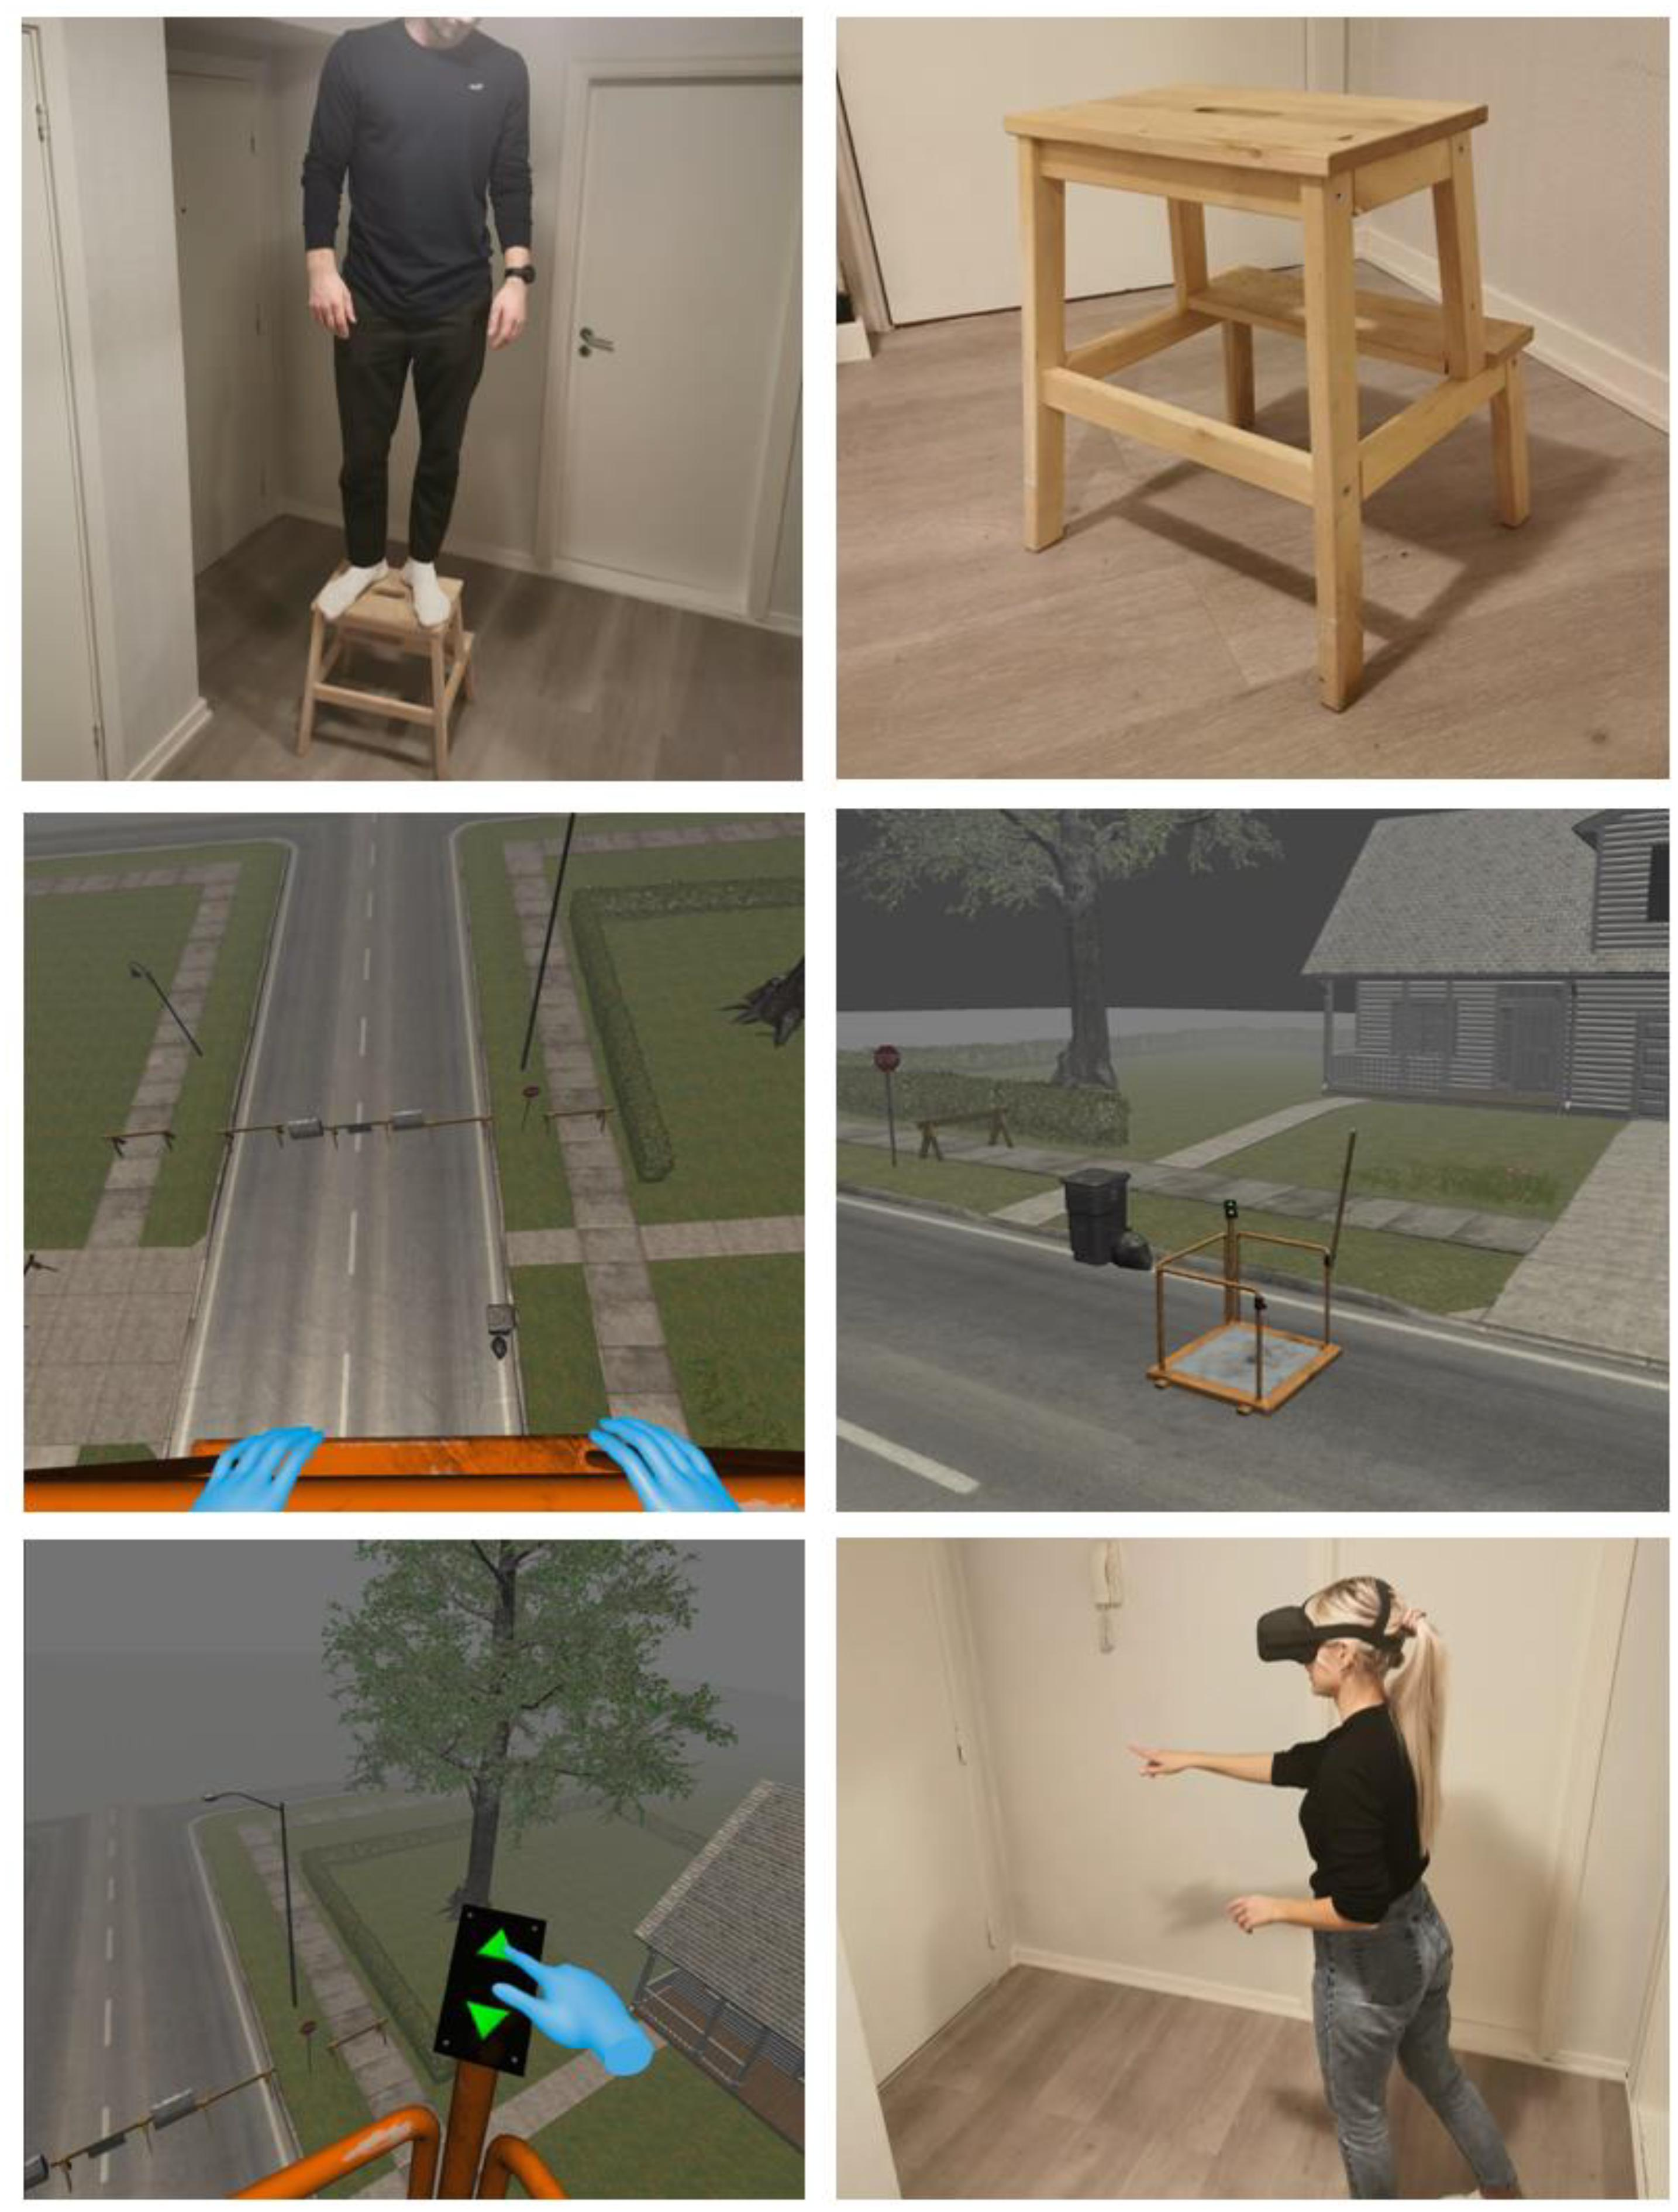
\includegraphics[width=0.6\linewidth]{capitulos/figuras/fear_of_heights.jpg}
    \caption{Exemplo de aplicação que usa \acrshort{RV} no tratamento da acrofobia \cite{Edwards2018}.}
    \label{fig:medoAltura}
\end{figure}

A indústria do entretenimento através de filmes e jogos provocou uma grande evolução de técnicas de \acrshort{RV} que posteriormente foram aplicadas em áreas mais “sérias” como o desenvolvimento pessoal e treinamento \cite{Ma2011, Prensky2001, Smith2011}. Na prática a \acrshort{RV} deve ser considerada como uma possibilidade sempre que o que se deseja fazer é muito perigoso, caro ou impraticável de ser realizado concretamente. Por conta destas características ela é muito usada nas áreas da educação, da saúde e militar \cite{VRS2018}. Conforme a tecnologia que permite a criação e simulação de ambientes virtuais se torna mais barata, mais aplicações são criadas com o uso destas ferramentas.

\section{Dispositivos Hápticos}

O termo \textit{haptics} é usado para descrever a ciência que estuda e simula a pressão, textura, vibração e outras sensações biológicas relacionadas ao toque. A sensação do toque se origina em estímulos mecânicos, elétricos, térmicos ou químicos na pele \cite{Burdea1996}. O tato não está localizado numa região específica do corpo como os demais sentidos. Ele está distribuído por todo o corpo através do órgão sensorial do toque, nossa pele, articulações, músculos e tendões. O senso do toque se divide em duas sensações: cinética e tátil. Forças e torques são sensações cinéticas que sentimos nos músculos, tendões e articulações. Já as sensações táteis como pressão, deformação e vibração são sentidas por mecano receptores que possuímos na nossa pele \cite{Culbertson2018}. 

Os primeiros dispositivos hápticos foram originados dos braços robóticos usados para o controle remoto de robôs \cite{Zurawski2005} As aplicações de tecnologias hápticas são muito variadas envolvendo, por exemplo, projetos de engenharia e aplicações de manufatura \cite{Sharma2001}, entretenimento (videogames e filmes), celulares, relógios inteligentes e até mesmo a indústria automobilística \cite{Smith2019}. Estes dispositivos possuem elementos mecânicos de entrada e saída para interação com o usuário. Uma ou mais partes do dispositivo em contato com o usuário são monitorados no espaço físico e o dispositivo oferece como retorno força e torque. Desta forma um canal bidirecional de interação entre o ambiente virtual e o usuário é criado \cite{Coles2011}. Estes dispositivos estão sendo cada vez mais utilizados hoje em dia tanto pela evolução da sua tecnologia como pela diminuição dos preços. Com o avanço da tecnologia estes dispositivos estão se tornando cada vez mais flexíveis representando mais fielmente os movimentos. Isto ocorre  através do uso de conceitos de restrição parcial a movimentos, deslocamentos e da inclusão de mais graus de liberdade, \textit{\acrfull{DoF}}. 

O número de graus de liberdade de um dispositivo háptico se refere ao número de maneiras diferentes em que este pode se mover ou criar forças. Como exemplo, dispositivos com 3 graus de liberdade podem rastrear posições e criar forças ao serem movidos nas direções: direita-esquerda, frente-trás e cima-baixo \cite{HAPTICSHOUSE2019}. O principal objetivo no uso destes dispositivos é o aumento da sensação de imersão em um ambiente de realidade virtual. 

Em relação à área médica, os dispositivos hápticos vem sendo utilizados na maioria dos trabalhos de simulação de procedimentos médicos \cite{Coles2011,Escobar-Castillejos2016}. Eles são usados para simular o uso de ferramentas em cirurgias e ajudaram a impulsionar o sucesso das práticas em simuladores virtuais. Isto aconteceu ao proporcionar o controle dos graus de liberdade de deslocamentos, a restrição aos movimentos e as respostas às atitudes do usuário como forças de reação ou \textit{feedback} \cite{Gerovich2004}. Estes dispositivos eletromecânicos existem nas mais diversas formas e são adaptados para uma grande variedade de procedimentos médicos como, por exemplo, no treinamento de laparoscopia \cite{Srinivasan2004}, biopsia de próstata \cite{Sclaverano2009}, cirurgia de fígado \cite{Mastmeyer2016}, exames de mama \cite{Brazil2017,Jeon2010,Ribeiro2014,Solanki2010}, simulação de apalpação \cite{Ribeiro2016} e punções epidurais \cite{N.2013, Brazil2018}. Alguns sistemas usam mais de um háptico como em punções de agulha guiadas por ultrassom que usam um equipamento para simular a agulha e outro para o ultrassom \cite{Ni2011,Vidal2008}. Outros chegam a fazer o uso de três dispositivos como o PalpSim de forma a simular o toque das mãos do usuário num paciente virtual \cite{Coles2011b}. 

\textcite{Culbertson2018} identificaram como 3 as principais categorias de sistemas hápticos: compreensíveis, vestíveis e palpáveis. Um exemplo visual destes tipos pode ser visto na Figura~\ref{fig:tiposHapticos}. Os sistemas compreensíveis são dispositivos tipicamente cinéticos (\textit{feedback} de força) que normalmente possuem uma base fixa e permitem ao usuário empurrar e ser empurrado de volta. Sistemas vestíveis são tipicamente táteis montados nas mãos ou em outras partes do corpo e provocam sensações diretamente na pele. Os sistemas palpáveis são dispositivos de encontro que permitem ao usuário explorar toda a superfície \cite{Culbertson2018}. Os dispositivos a serem explorados aqui são os de sistemas compreensíveis. Estes foram os tipos de hápticos utilizados nos simuladores computacionais relacionados ao tema desta tese \ref{sec:simuladoresComputacionais} assim com nos diversos outros simuladores médicos estudados e citados nesta seção. \textcite{Ribeiro2016} fizeram uma revisão sobre dispositivos usados na simulação de procedimentos que envolvem o toque da mão do médico para identificação de características e anormalidades sob a pele. Os autores analisaram 57 trabalhos e mais da metade fez uso dos dispositivos da família \textit{Phantom}. Os dispositivos desta família serão listados nesta seção.

\begin{figure}[ht!]
    \centering
    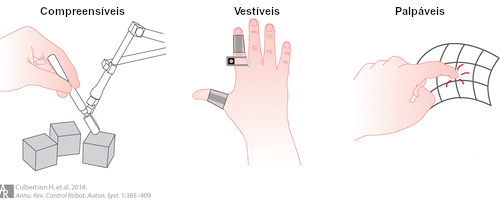
\includegraphics[width=0.6\linewidth]{capitulos/figuras/tipos.hapticos-portugues.png}
    \caption{Tipos de sistemas háptico \cite{Culbertson2018}.}
    \label{fig:tiposHapticos}
\end{figure}

Nas figuras~\ref{fig:hapticoNovintFalcon}, \ref{fig:hapticoTouch}, \ref{fig:hapticoTouchX} e  \ref{fig:hapticoPremium}, os dispositivos aparecem representados ordenados pelas suas complexidades i.e. dos mais simples (mais antigos e com menos recursos) aos mais avançados (mais novos). Todos estes dispositivos são exemplos de sistemas tipicamente cinéticos. Os mais novos possibilitam maior número de graus de liberdade para os movimentos assim como possibilitam mais forças e momentos de reação. O Novint Falcon ® (Figura~\ref{fig:hapticoNovintFalcon}), lançado em 2007, tem como interface com o usuário uma esfera onde o usuário deve colocar os dedos da mão para fazer os movimentos no caso do seu uso mais comum. No que diz respeito à liberdade de movimento este mecanismo proporciona uma interação 3D com o computador no lugar da interação 2D proporcionada pelo mouse. Ele possui 3 graus de liberdade de movimento e de forças. Nesta esfera existem quatro botões para interação e existem sensores para determinar a posição do cursor e motores para controlar as forças a serem transmitidas para o usuário. Existem versões onde a esfera é substituída, por exemplo, por um dispositivo semelhante a uma pistola para que o dispositivo seja usado em jogos de tiros de primeira pessoa \cite{VRS2017}. 

\begin{figure}[ht!]
    \centering
    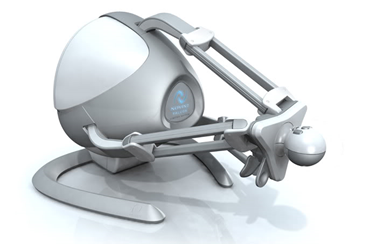
\includegraphics[width=0.4\linewidth]{capitulos/figuras/hapticoNovintFalcon.png}
    \caption{Dispositivo háptico Novint Falcon ® \cite{HAPTICSHOUSE2019}
    \label{fig:hapticoNovintFalcon}.}
\end{figure}

\begin{figure}[ht!]
    \centering
    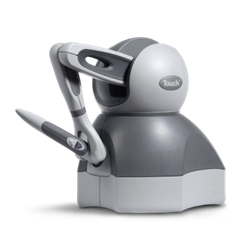
\includegraphics[width=0.4\linewidth]{capitulos/figuras/hapticoTouch.png}
    \caption{Dispositivo háptico Geomagic Touch ® / Phantom Omni ® \cite{3DSystems2018}.}
    \label{fig:hapticoTouch}
\end{figure}

\begin{figure}[ht!]
    \centering
    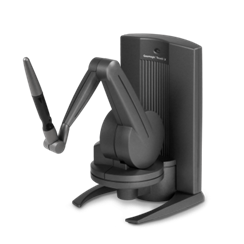
\includegraphics[width=0.4\linewidth]{capitulos/figuras/hapticoTouchX.png}
    \caption{Dispositivo háptico Geomagic Touch X ® / Phantom Desktop ® \cite{3DSystems2018}.}
    \label{fig:hapticoTouchX}
\end{figure}


\begin{figure}[ht!]
    \centering
    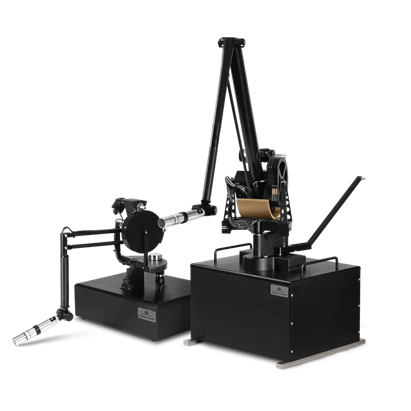
\includegraphics[width=0.4\linewidth]{capitulos/figuras/hapticoPhantomPremium.png}
    \caption{Dispositivo háptico Phantom Premium ® \cite{3DSystems2018}.}
    \label{fig:hapticoPremium}
\end{figure}

Os hápticos da família \textit{Phantom Geomagic Touch} ® (Figura~\ref{fig:hapticoTouch}) e \textit{Geomagic Touch} X ® (Figura~\ref{fig:hapticoTouchX}) apresentam uma peça que simula uma caneta para manipulação do usuário da mesma forma que a esfera no dispositivo da Figura~\ref{fig:hapticoNovintFalcon}. Nas canetas também existem botões para interação e da mesma forma estas também são substituíveis por partes com formas mais adequadas ao procedimento que estas pretendem simular. O dispositivo \textit{Geomagic Touch} X ® possui a mesma liberdade de movimento do \textit{Geomagic Touch} ®, porém possibilita \textit{feedback} de reações maiores. Ambos apresentam 6 graus de liberdade de movimento e 3 graus de liberdade no retorno de forças. Estes dispositivos, portanto mapeiam a posição 3D e orientação, mas somente apresentam \textit{feedback} de forças direcionais \cite{Forsslund2013}.

O \textit{Phantom Premium} ® (Figura~\ref{fig:hapticoPremium}) está disponível nas versões \textit{Premium} 1.0, \textit{Premium 1.5} e 1.5/HF, e \textit{Premium} 3.0. Estas evoluem não só o \textit{feedback} de reações como também os graus de liberdade dos movimentos. Enquanto o \textit{Phantom Premium} 1.0 ® simula o movimento do giro do pulso na mão o \textit{Phantom Premium} 3.0 ® possibilita uma amplitude que simula os graus de liberdade de movimento de todo o braço humano desde o ombro \cite{3DSystems2018}. Este dispositivo possui 6 graus de liberdade tanto para movimento como retorno de forças o que o torna simétrico no número de sensores e motores (atuadores). São computadas forças e torques tanto da posição como da orientação deste dispositivo. Esta característica tem uma forte influencia no alto custo associado a este tipo de dispositivo \cite{Forsslund2013}.

\section{Modelagem de tecidos}

Um dos passos necessários para construção de um ambiente virtual para treinamento de anestesia epidural e raquianestesia é a criação de pacientes virtuais. Um importante aspecto da modelagem destes pacientes é como eles aparecem na tela da aplicação. Outro aspecto importante na simulação é ter uma estimativa da espessura dos tecidos envolvidos nestes tipos de anestesia. Para isto é necessária à modelagem do tamanho de todas as camadas de tecido pelos quais as agulhas passam para execução destes procedimentos. Uma ilustração destes tecidos que vão desde a pele até a dura-máter pode ser vista na Figura 3. Nesta seção são descritos trabalhos relacionados com a modelagem da distância entre a pele e a dura-máter.

Na Tabela 2 são listadas as varáveis de entrada e saída dos métodos estudados nesta seção. Esta tabela exibe também as unidades destas variáveis que serão utilizadas em todo este trabalho.

===== TABELA ====

Muitos trabalhos buscam relacionar a distância que vai da superfície externa da pele até o espaço epidural (DEE) com as demais variáveis da Tabela 2. A grande maioria dos trabalhos indica uma forte relação da DEE com o IMC \cite{Adegboye2017, Galbraith2018}. Estes dois trabalhos não fazem separação dos grupos populacionais por idade, sexo ou etnia, e usaram populações respectivamente de n=120 e n=317 pessoas entre homens e mulheres.

Os trabalhos citados a seguir analisaram somente ou de forma separada grupos de mulheres grávidas. Como este é o foco deste trabalho só serão comentadas aqui as conclusões referentes a estes grupos. Todos os trabalhos a seguir encontraram influencia do IMC na determinação da DEE, mas além desta relação também foram encontradas outras combinações em cada trabalho. O grupo étnico/populacional do individuo foi observado em conjunto com o IMC em \cite{Sharma2011} estudo feito no Reino Unido. A idade foi observada em conjunto com o IMC num estudo em pacientes americanas em Michigan, EUA \cite{Clinkscales2007}. A altura, massa, idade e IMC foram observados como relevantes em um estudo em pacientes da Índia \cite{Hazarika2016}. Estes dois últimos trabalhos construíram equações de regressão linear para determinação da DEE para grupos de parturientes conforme pode ser visto na Tabela 3.

===== TABELA ====

Os autores em \cite{Sharma2011} no lugar das equações apresentaram como resultado uma tabela com cinco pontos de cada par IMC x DEE para cada grupo populacional analisado. Estes dados podem ser vistos na Tabela 4. A definição dos grupos populacionais no estudo do Reino Unido (RU) em \cite{Sharma2011} foi: Brancas (população do Reino Unido, da Irlanda e qualquer outro grupo com cor de pele branca); Asiáticas ou Britânicas Asiáticas (população da Índia, Paquistão, Bangladesh ou qualquer outro grupo Asiático); Negras ou Britânicas negras (população de Africanas, Caribenhas ou outros grupos com cor da pele negra); e Chinesas e outros grupos étnicos (população da China, Japão, Malásia, Filipinas etc.). No grupo de nome Chinesas, além dos dados de pessoas desta origem moradoras do Reino Unido, foram considerados dados de Chinesas (n=70) de um hospital de Singapura.

===== TABELA ====

Na Tabela 5 é apresentado o tamanho da população utilizada nestes estudos e as identificações da origem dos dados do estudo, isto é, os grupos populacionais analisados. 

===== TABELA ====

A listagem dos tecidos entre a pele e a DEE e a relação dessa distância com o aumento de peso é comentada em \cite{Palmer1983}. Os autores concluem que com o aumento do peso/massa (do paciente) o tecido que sofre a maior variação é a gordura subcutânea.

Na seção = ==== é proposto o uso de dados de trabalhos comentados aqui para modelagem de tecidos de pacientes grávidas.

=========

Este capítulo apresentou uma fundamentação teórica sobre ====. Iniciou apresentando ==========. Logo em seguida o capítulo apresenta ====== e suas principais entidades e que estão relacionadas com a proposta desta tese. O capitulo finaliza apresentando os conceitos que envolvem ==== e seus principais elementos. O próximo capítulo oferece uma visão das pesquisas relacionadas ao tema desta tese e compara-as com as proposições que foram colocadas ao longo deste trabalho. Essas pesquisas tratam e ========== assim como de ===========.